\documentclass[12pt,a4paper]{article}
\usepackage[utf8]{vietnam}
\usepackage{amsmath,amssymb,amsfonts,mathrsfs}
\usepackage[left=1.5cm,right=1.5cm,top=2cm,bottom=2cm,headheight=17pt]{geometry}
\usepackage{enumitem}
\usepackage{array}
\usepackage{graphicx}
\usepackage{fancyhdr}

\pagestyle{fancy}
\fancyhf{}
\lhead{\small\textbf{HƯỚNG TỚI THPTQG 2027}}
\rhead{\small\textit{Người biên soạn: Dương Gia Bảo}}
\rfoot{\small Trang \thepage}
\renewcommand{\headrulewidth}{0.4pt}

\begin{document}

\noindent
\begin{minipage}[t]{0.40\textwidth}
    \centering
    \textbf{HƯỚNG TỚI THPTQG 2027}\\[-2pt]
    \rule{3.2cm}{0.6pt}\\[4pt]
    \textbf{ĐỀ CHÍNH THỨC}
\end{minipage}\hfill
\begin{minipage}[t]{0.58\textwidth}
    \centering
    \textbf{ĐỀ THI KHẢO SÁT CHẤT LƯỢNG}\\
    \textbf{ĐỀ SỐ 3}\\
    \textbf{Môn thi: TOÁN}\\
    \textit{\small Thời gian làm bài: 90 phút, không kể thời gian phát đề}
\end{minipage}

\vspace{0.2cm}
\noindent
\begin{minipage}[b]{0.78\textwidth}
    \textbf{Họ và tên:}\dotfill\textbf{SBD:}\makebox[3.5cm]{\dotfill}
\end{minipage}\hfill
\begin{minipage}[b]{0.20\textwidth}
    \hfill
    \setlength{\fboxrule}{0.8pt}%
    \fbox{\begin{minipage}{2.3cm}
        \centering
        \textbf{\small Mã đề thi}\\
        \textbf{0003}
    \end{minipage}}
\end{minipage}
\vspace{0.2cm}

% ==========================================
% PHẦN I
% ==========================================
\section*{\large PHẦN I. CÂU TRẮC NGHIỆM NHIỀU PHƯƠNG ÁN LỰA CHỌN}
\textit{Thí sinh trả lời từ câu 1 đến câu 12. Mỗi câu hỏi thí sinh chỉ chọn một phương án. Mỗi câu trả lời đúng được 0,25 điểm.}

\begin{enumerate}[label=\textbf{Câu \arabic*:}, leftmargin=*]

\item Cho hàm số $y = \dfrac{x^2 - (m+2)x + 2m}{x - 1}$ có đồ thị là $(C_m)$ (với $m$ là tham số thực). Gọi $S$ là tập hợp tất cả các giá trị của tham số $m$ để đồ thị $(C_m)$ có hai điểm cực trị $A, B$ sao cho tam giác $OAB$ vuông tại gốc tọa độ $O$. Tổng các phần tử của tập hợp $S$ bằng
\begin{enumerate}[label=\Alph*.]
    \item $5$.
    \item $6$.
    \item $-5$.
    \item $1$.
\end{enumerate}

\item Có bao nhiêu giá trị nguyên của tham số $m \in [-20; 20]$ để bất phương trình $\log_3(x^2 + 1) + 1 \ge \log_3(x^2 + 2x + m)$ nghiệm đúng với mọi số thực $x \in \mathbb{R}$?
\begin{enumerate}[label=\Alph*.]
    \item $0$.
    \item $1$.
    \item $2$.
    \item $3$.
\end{enumerate}

\item Cho hàm số $f(x)$ liên tục và không âm trên đoạn $[0; 1]$ thỏa mãn $f(x) + x f'(x) = (x + 1)e^x$ với mọi $x \in [0; 1]$ và $f(1) = e$. Tính tích phân $I = \int_0^1 f(x) dx$.
\begin{enumerate}[label=\Alph*.]
    \item $I = e - 1$.
    \item $I = \dfrac{e - 1}{3}$.
    \item $I = \dfrac{e + 1}{2}$.
    \item $I = e + 1$.
\end{enumerate}

\item Trong không gian $Oxyz$, cho mặt cầu $(S): x^2 + y^2 + z^2 - 2x + 4y - 6z + 5 = 0$ và hai điểm $A(1; 0; 1)$, $B(2; -1; 2)$. Gọi $M(a; b; c)$ là điểm thuộc mặt cầu $(S)$ sao cho biểu thức $P = MA^2 + 2MB^2$ đạt giá trị nhỏ nhất. Tính tổng $T = a + b + c$.
\begin{enumerate}[label=\Alph*.]
    \item $T = 3$.
    \item $T = \dfrac{1}{3}$.
    \item $T = -\dfrac{5}{3}$.
    \item $T = 1$.
\end{enumerate}

\item Cho cấp số nhân $(u_n)$ có các số hạng đều dương, thỏa mãn $u_1 > 0$ và công bội $q > 0$. Biết $u_2 \cdot u_4 = 16$. Biểu thức $P = 16u_1 + u_5$ đạt giá trị nhỏ nhất khi công bội $q$ bằng
\begin{enumerate}[label=\Alph*.]
    \item $q = \sqrt{2}$.
    \item $q = 2$.
    \item $q = \sqrt{3}$.
    \item $q = \dfrac{1 + \sqrt{5}}{2}$.
\end{enumerate}

\item Khảo sát thời gian hoàn thành bài thi năng khiếu (đơn vị: phút) của $100$ thí sinh thu được mẫu số liệu ghép nhóm sau:
\begin{center}
\begin{tabular}{|c|c|c|c|c|c|}
\hline
\textbf{Thời gian (phút)} & $[10; 15)$ & $[15; 20)$ & $[20; 25)$ & $[25; 30)$ & $[30; 35)$ \\ \hline
\textbf{Số thí sinh} & $12$ & $28$ & $35$ & $17$ & $8$ \\ \hline
\end{tabular}
\end{center}
Khoảng tứ phân vị $\Delta_Q = Q_3 - Q_1$ của mẫu số liệu ghép nhóm trên bằng (làm tròn đến hàng phần trăm)
\begin{enumerate}[label=\Alph*.]
    \item $7{,}68\text{ phút}$.
    \item $6{,}88\text{ phút}$.
    \item $7{,}25\text{ phút}$.
    \item $6{,}50\text{ phút}$.
\end{enumerate}

\item Hai dây chuyền máy móc sản xuất linh kiện điện tử hoạt động độc lập. Tỉ lệ phế phẩm do dây chuyền I tạo ra là $3\%$, do dây chuyền II tạo ra là $5\%$. Lấy ngẫu nhiên $1$ sản phẩm từ dây chuyền I và $2$ sản phẩm từ dây chuyền II. Xác suất để trong $3$ sản phẩm lấy ra có đúng $1$ phế phẩm bằng (làm tròn đến hàng phần vạn)
\begin{enumerate}[label=\Alph*.]
    \item $0{,}1192$.
    \item $0{,}1215$.
    \item $0{,}0925$.
    \item $0{,}1025$.
\end{enumerate}

\item Cho hàm số $y = \dfrac{\sqrt{x^2 - 4}}{x^2 - (m+2)x + 2m}$. Có bao nhiêu giá trị nguyên của $m \in [-10; 10]$ để đồ thị hàm số có đúng $3$ đường tiệm cận?
\begin{enumerate}[label=\Alph*.]
    \item $17$.
    \item $18$.
    \item $16$.
    \item $15$.
\end{enumerate}

\item Cho hình phẳng $(H)$ giới hạn bởi đồ thị hàm số $y = x \sqrt{\ln(x + 1)}$, trục hoành và đường thẳng $x = 1$. Thể tích $V$ của khối tròn xoay thu được khi quay hình phẳng $(H)$ xung quanh trục $Ox$ bằng
\begin{enumerate}[label=\Alph*.]
    \item $V = \pi \left( \dfrac{2}{3} \ln 2 - \dfrac{5}{18} \right)$.
    \item $V = \pi \left( \dfrac{1}{3} \ln^2 2 - \dfrac{1}{9} \right)$.
    \item $V = \pi \left( \dfrac{4}{3} \ln 2 - \dfrac{7}{9} \right)$.
    \item $V = \pi \left( \dfrac{2}{3} \ln 2 - \dfrac{1}{6} \right)$.
\end{enumerate}

\item Trong không gian $Oxyz$, cho hai đường thẳng $d_1: \dfrac{x-1}{2} = \dfrac{y+1}{1} = \dfrac{z}{-1}$ và $d_2: \dfrac{x-2}{1} = \dfrac{y-3}{-2} = \dfrac{z+1}{2}$. Khoảng cách giữa hai đường thẳng $d_1$ và $d_2$ bằng
\begin{enumerate}[label=\Alph*.]
    \item $\dfrac{3\sqrt{2}}{2}$.
    \item $\sqrt{10}$.
    \item $\dfrac{\sqrt{30}}{3}$.
    \item $3$.
\end{enumerate}

\item Cho bất phương trình $9^x - m \cdot 3^{x+1} + 2m + 1 \le 0$. Tìm tất cả các giá trị nguyên của tham số $m \in [-10; 10]$ để bất phương trình có nghiệm thuộc đoạn $[0; 1]$.
\begin{enumerate}[label=\Alph*.]
    \item $10$.
    \item $9$.
    \item $11$.
    \item $8$.
\end{enumerate}

\item Trong không gian $Oxyz$, cho hai điểm $A(1; 2; 1)$, $B(3; 0; -1)$ và đường thẳng $d: \dfrac{x-1}{1} = \dfrac{y}{2} = \dfrac{z+1}{-2}$. Tọa độ điểm $M$ thuộc đường thẳng $d$ sao cho biểu thức $P = MA^2 + MB^2$ đạt giá trị nhỏ nhất là
\begin{enumerate}[label=\Alph*.]
    \item $M\left(\dfrac{10}{9}; \dfrac{2}{9}; -\dfrac{11}{9}\right)$.
    \item $M(1; 0; -1)$.
    \item $M(2; 2; -3)$.
    \item $M(0; -2; 1)$.
\end{enumerate}

\end{enumerate}

% ==========================================
% PHẦN II
% ==========================================
\section*{PHẦN II. CÂU TRẮC NGHIỆM ĐÚNG/SAI}
\textit{Thí sinh trả lời từ câu 1 đến câu 4. Trong mỗi ý a), b), c), d) ở mỗi câu, thí sinh chọn Đúng hoặc Sai.}

\begin{enumerate}[label=\textbf{Câu \arabic*:}, leftmargin=*]

\item Một nhà máy hóa chất sản xuất xút (NaOH) phục vụ ngành công nghiệp. Tổng chi phí sản xuất $x$ tấn xút mỗi ngày ($x > 0$) được xác định bởi hàm số $C(x) = 0{,}1x^3 - 3x^2 + 40x + 100$ (triệu đồng). Giá bán mỗi tấn xút phụ thuộc vào lượng cung ứng ra thị trường theo hàm giá $p(x) = 100 - 2x$ (triệu đồng/tấn). Doanh nghiệp thu được lợi nhuận hàng ngày là $L(x) = R(x) - C(x)$, trong đó $R(x) = x \cdot p(x)$ là tổng doanh thu bán $x$ tấn xút.
\begin{center}
    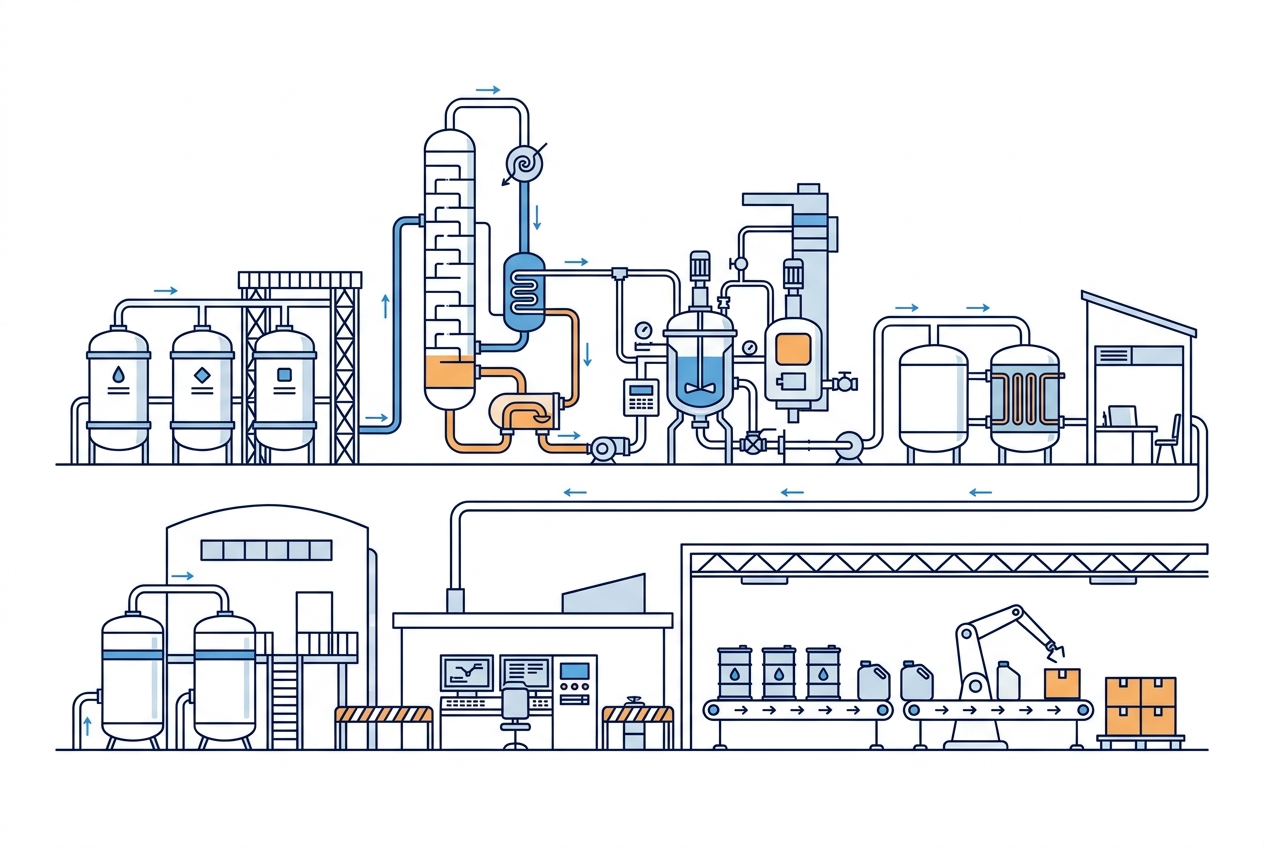
\includegraphics[width=0.42\linewidth,height=3.2cm,keepaspectratio]{images/phan2_cau1_nhamayxut.jpg}
\end{center}
\begin{enumerate}[label=\alph*)]
    \item Hàm doanh thu bán $x$ tấn xút mỗi ngày là $R(x) = 100x - 2x^2$ (triệu đồng).
    \item Hàm lợi nhuận hàng ngày của nhà máy được biểu diễn bởi $L(x) = -0{,}1x^3 + x^2 + 60x - 100$ (triệu đồng).
    \item Khi nhà máy sản xuất $10$ tấn xút mỗi ngày thì lợi nhuận thu được là $500$ triệu đồng.
    \item Doanh nghiệp đạt lợi nhuận lớn nhất khi sản xuất $x = 18$ tấn xút mỗi ngày và mức lợi nhuận lớn nhất đạt được bằng $718{,}8$ triệu đồng.
\end{enumerate}

\item Một hệ thống pin năng lượng mặt trời thông minh tự động xoay tấm pin để đón ánh nắng. Tốc độ thu năng lượng điện (đơn vị: kW) trong một ngày nắng kéo dài $12$ giờ ($0 \le t \le 12$) được mô hình hóa bởi hàm số $f(t) = -0{,}15t^2 + 1{,}8t$ (kW), trong đó $t = 0$ tương ứng thời điểm $6$ giờ sáng. Gọi $F(t)$ là tổng năng lượng điện thu được (đơn vị: kWh) kể từ $t = 0$ đến thời điểm $t$, thỏa mãn $F(0) = 0$ và $F'(t) = f(t)$.
\begin{center}
    
\includegraphics[width=0.42\linewidth,height=3.2cm,keepaspectratio]{images/phan2_cau2_pinmattroi.jpg}
\end{center}
\begin{enumerate}[label=\alph*)]
    \item Tốc độ thu năng lượng điện của hệ thống đạt giá trị lớn nhất tại thời điểm $t = 6$ (tương ứng $12$ giờ trưa).
    \item Tổng năng lượng điện hệ thống thu được trong $6$ giờ đầu tiên (từ $6$ giờ sáng đến $12$ giờ trưa) bằng $16{,}2\text{ kWh}$.
    \item Tổng năng lượng điện hệ thống thu được trong suốt $12$ giờ chiếu sáng của ngày hôm đó bằng $43{,}2\text{ kWh}$.
    \item Để thu được $80\%$ tổng năng lượng điện của cả ngày, hệ thống cần hoạt động liên tục từ $6$ giờ sáng đến khoảng $14$ giờ $30$ phút cùng ngày.
\end{enumerate}

\item Một bệnh viện lớn sử dụng phần mềm trí tuệ nhân tạo (AI) để tầm soát sớm một loại ung thư hiếm gặp trong cộng đồng. Tỉ lệ người mắc bệnh này trong dân số hiện tại là $0{,}5\%$. Mô hình AI có độ nhạy $96\%$ (người mắc bệnh AI chẩn đoán dương tính $96\%$) và tỉ lệ dương tính giả $2\%$ (người không mắc bệnh AI chẩn đoán lầm dương tính $2\%$). Khi AI báo kết quả dương tính, bệnh nhân tiếp tục được xét nghiệm sinh thiết chuyên sâu với độ chính xác $98\%$ (âm tính giả $2\%$).
\begin{center}
    
\includegraphics[width=0.42\linewidth,height=3.2cm,keepaspectratio]{images/phan2_cau3_aitamsoat.jpg}
\end{center}
\begin{enumerate}[label=\alph*)]
    \item Xác suất một người chọn ngẫu nhiên trong cộng đồng không mắc bệnh là $99{,}5\%$.
    \item Xác suất một người chọn ngẫu nhiên trong cộng đồng có kết quả AI chẩn đoán dương tính là $P(B) = 0{,}0247$ (tức $2{,}47\%$).
    \item Nếu một người chọn ngẫu nhiên có kết quả AI chẩn đoán dương tính, xác suất người đó thực sự mắc bệnh xấp xỉ $19{,}4\%$.
    \item Nếu một người trải qua cả hai vòng (AI chẩn đoán dương tính và xét nghiệm sinh thiết chuyên sâu cũng cho kết quả dương tính), xác suất người đó thực sự mắc bệnh đạt trên $90\%$.
\end{enumerate}

\item Một tấm sàn bê tông phẳng đồng chất hình chữ nhật $ABCD$ có khối lượng $M = 300\text{ kg}$ được nâng cân bằng trong công trường xây dựng nhờ bốn sợi dây cáp thép nhẹ không giãn $SA, SB, SC, SD$ chăng từ móc cẩu $S(0; 0; 6)$ xuống bốn góc sàn $A(-2; -3; 0)$, $B(2; -3; 0)$, $C(2; 3; 0)$, $D(-2; 3; 0)$ đặt trong hệ tọa độ $Oxyz$ (đơn vị đo trên các trục là mét). Lấy $g = 10\text{ m/s}^2$. Trọng lực tác dụng tại tâm $O(0; 0; 0)$ là $\vec{P} = (0; 0; -3000)\text{ (N)}$.
\begin{center}
    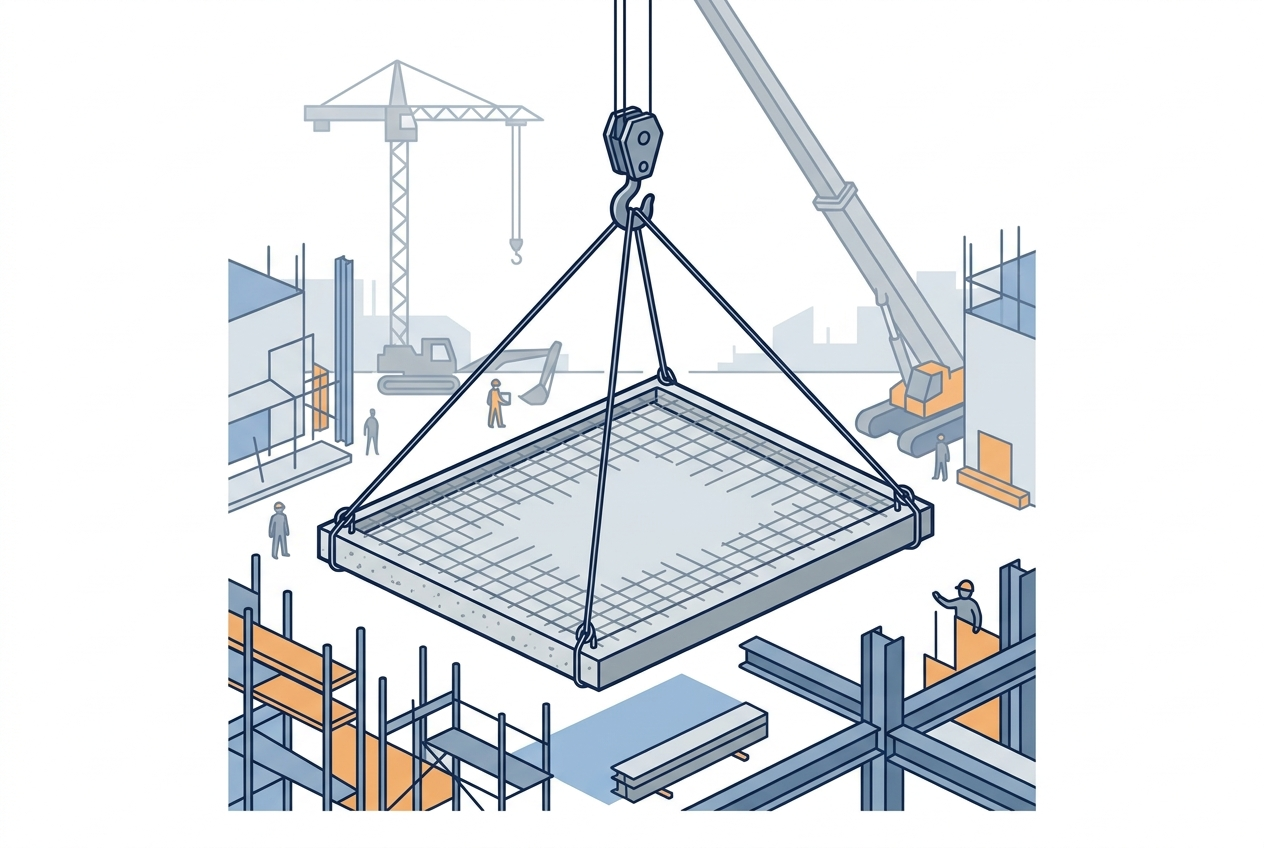
\includegraphics[width=0.42\linewidth,height=3.2cm,keepaspectratio]{images/phan2_cau4_sancap.jpg}
\end{center}
\begin{enumerate}[label=\alph*)]
    \item Tọa độ vectơ $\overrightarrow{SA} = (-2; -3; -6)$ và độ dài $|\overrightarrow{SA}| = 7\text{ m}$.
    \item Độ dài của cả bốn sợi dây cáp $SA, SB, SC, SD$ đều bằng nhau và bằng $7\text{ m}$.
    \item Do tính đối xứng và điều kiện cân bằng lực $\vec{F}_1 + \vec{F}_2 + \vec{F}_3 + \vec{F}_4 + \vec{P} = \vec{0}$, lực căng trên mỗi sợi dây cáp bằng $875\text{ N}$.
    \item Góc tạo bởi dây cáp $SA$ và mặt phẳng sàn $(ABCD)$ xấp xỉ $59^\circ$.
\end{enumerate}

\end{enumerate}

% ==========================================
% PHẦN III
% ==========================================
\section*{PHẦN III. CÂU TRẮC NGHIỆM TRẢ LỜI NGẮN}
\textit{Thí sinh trả lời từ câu 1 đến câu 6. Điền đáp số theo quy chuẩn làm tròn được nêu trong từng câu.}

\begin{enumerate}[label=\textbf{Câu \arabic*:}, leftmargin=*]

\item Một doanh nghiệp cần xây dựng một bể chứa nước ngầm hình hộp chữ nhật có nắp đậy bằng bê tông với thể tích $V = 72\text{ m}^3$. Do điều kiện địa chất mặt bằng thi công, đáy bể bắt buộc phải có chiều dài gấp đôi chiều rộng. Đơn giá thi công hoàn thiện mặt đáy là $1$ triệu đồng/m$^2$, nắp bể là $1$ triệu đồng/m$^2$, và bốn mặt tường xung quanh là $1$ triệu đồng/m$^2$. Tìm chiều cao $h$ (đơn vị: mét) của bể để tổng chi phí vật liệu thi công làm bể là nhỏ nhất.
\begin{center}
    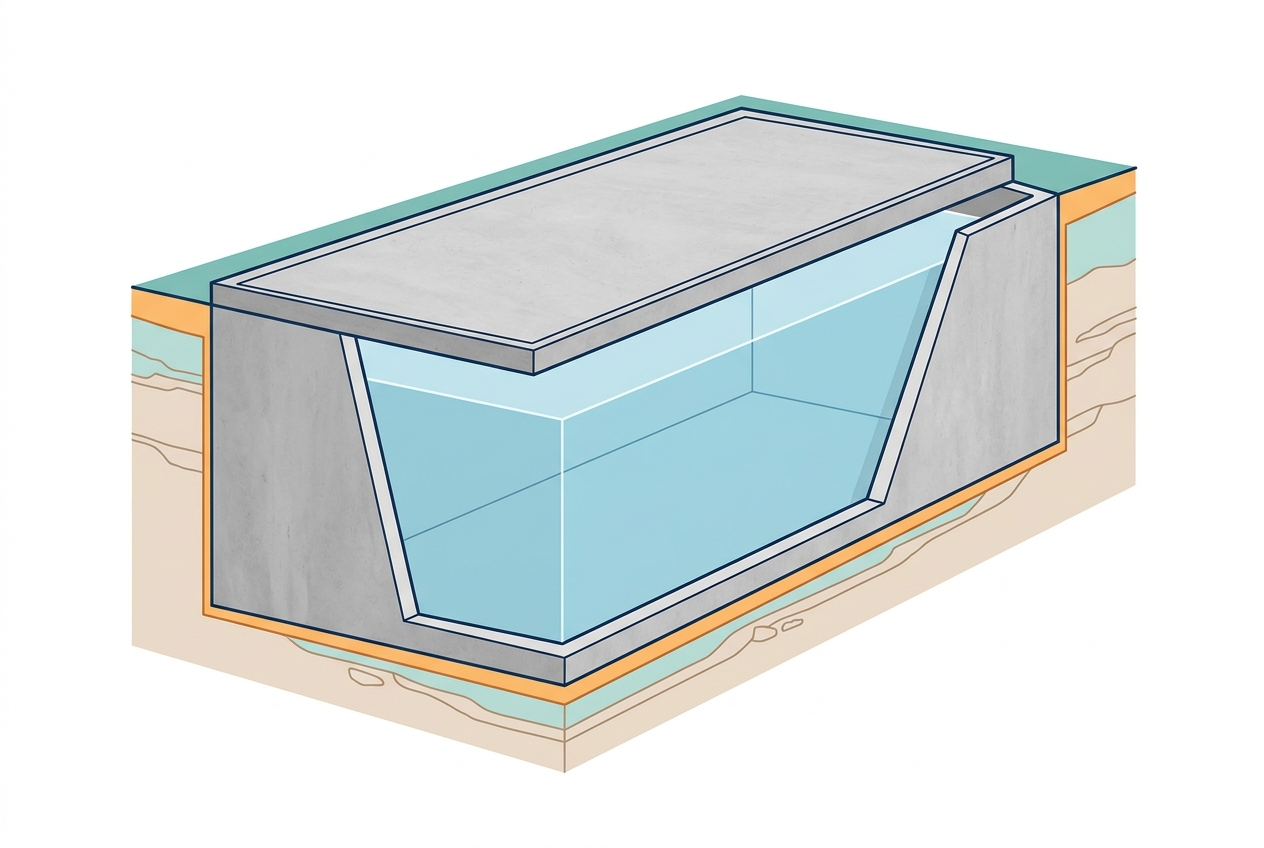
\includegraphics[width=0.42\linewidth,height=3.2cm,keepaspectratio]{images/phan3_cau1_bechuanuoc.jpg}
\end{center}

\item Một gia đình trẻ bắt đầu kế hoạch tích lũy tài chính để mua nhà. Vào ngày đầu tiên của mỗi tháng, gia đình gửi đều đặn số tiền $15$ triệu đồng vào tài khoản tiết kiệm ngân hàng áp dụng mức lãi suất $0{,}5\%$/tháng theo hình thức lãi kép (tiền lãi của tháng trước được tự động gộp vào tiền gốc tháng sau). Hỏi sau ít nhất bao nhiêu tháng gửi tiền thì tổng số tiền tích lũy được (cả gốc lẫn lãi) sẽ vượt quá $1$ tỷ đồng?
\begin{center}
    
\includegraphics[width=0.42\linewidth,height=3.2cm,keepaspectratio]{images/phan3_cau2_tietkiem.jpg}
\end{center}

\item Một nhân viên kiểm soát không lưu đang theo dõi hai thiết bị bay không người lái (drone) $A$ và $B$ tại trung tâm điều hành $O(0; 0; 0)$ trong hệ tọa độ $Oxyz$ (đơn vị đo là km). Tại thời điểm $t = 0$ (phút), drone $A$ ở vị trí $A_0(1; 2; 3)$ và di chuyển theo vectơ vận tốc $\vec{v}_A = (2; 1; 1)$ (km/phút); drone $B$ ở vị trí $B_0(5; 1; 1)$ và di chuyển theo vectơ vận tốc $\vec{v}_B = (1; 3; 2)$ (km/phút). Tìm khoảng cách ngắn nhất giữa hai drone trong quá trình bay (làm tròn kết quả đến hàng phần trăm của km).
\begin{center}
    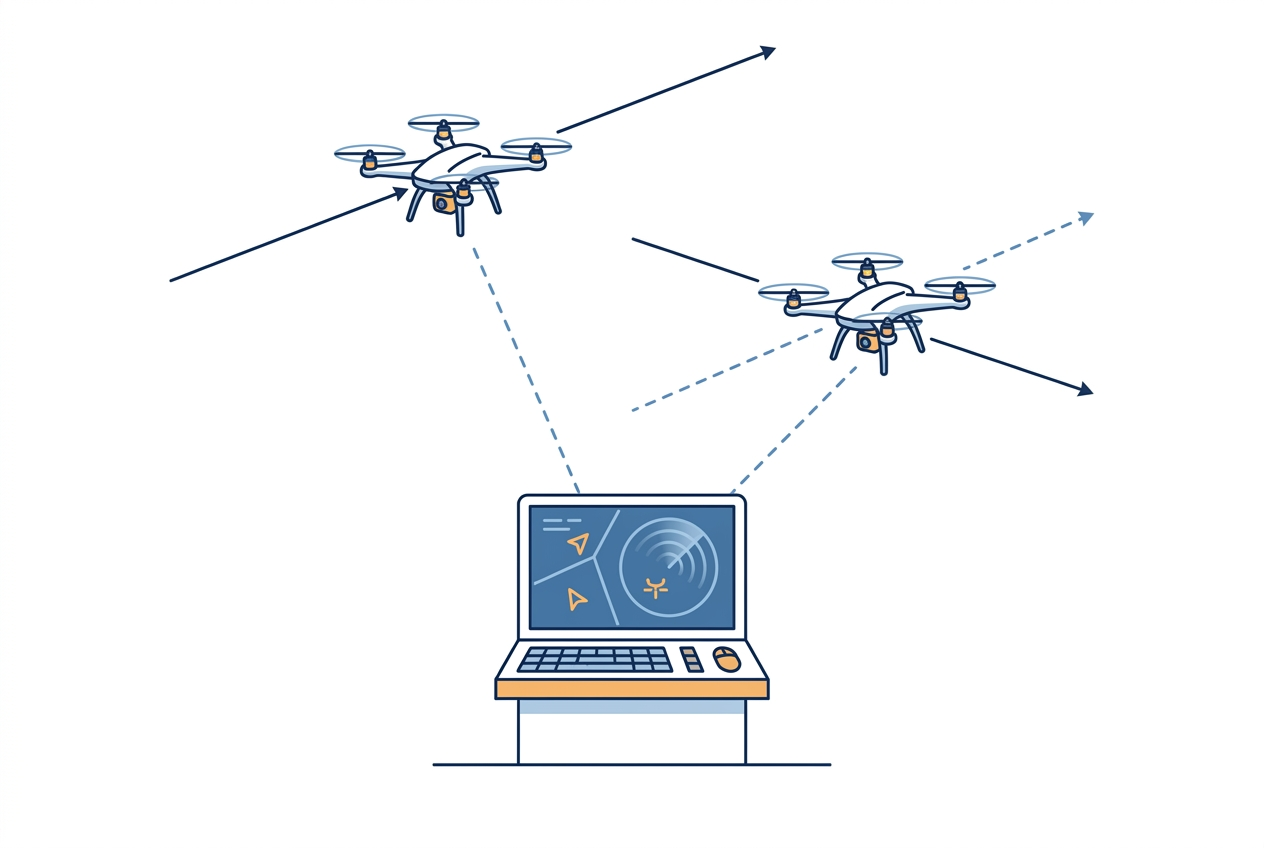
\includegraphics[width=0.42\linewidth,height=3.2cm,keepaspectratio]{images/phan3_cau3_drone.jpg}
\end{center}

\item Một kỹ sư nông nghiệp tiến hành khảo sát năng suất lúa (đơn vị: tạ/ha) tại $60$ hợp tác xã nông nghiệp. Kết quả thu được bảng tần số ghép nhóm sau:
\begin{center}
\begin{tabular}{|c|c|c|c|c|c|}
\hline
\textbf{Năng suất (tạ/ha)} & $[10; 12)$ & $[12; 14)$ & $[14; 16)$ & $[16; 18)$ & $[18; 20)$ \\ \hline
\textbf{Số hợp tác xã} & $8$ & $12$ & $x$ & $y$ & $6$ \\ \hline
\end{tabular}
\end{center}
Do tài liệu bị mờ, tần số $x$ và $y$ thuộc hai nhóm trung tâm bị mất. Biết rằng tổng số hợp tác xã là $60$ và trung vị của mẫu số liệu ghép nhóm là $M_e = 16{,}4$. Tìm giá trị của tần số $y$.

\item Một quản đốc xí nghiệp điện tử kiểm tra quy trình sản xuất linh kiện trên $3$ dây chuyền tự động $D_1, D_2, D_3$ với tỉ lệ sản lượng lần lượt là $50\%$, $30\%$ và $20\%$. Tỉ lệ hỏng của linh kiện do các dây chuyền $D_1, D_2, D_3$ tạo ra tương ứng là $1\%$, $2\%$ và $3\%$. Rút ngẫu nhiên một linh kiện từ kho hàng chung và phát hiện đây là một linh kiện bị hỏng. Tính xác suất để linh kiện bị hỏng này do dây chuyền $D_1$ sản xuất (làm tròn kết quả đến chữ số thập phân thứ hai dưới dạng số thập phân, ví dụ $0{,}29$).
\begin{center}
    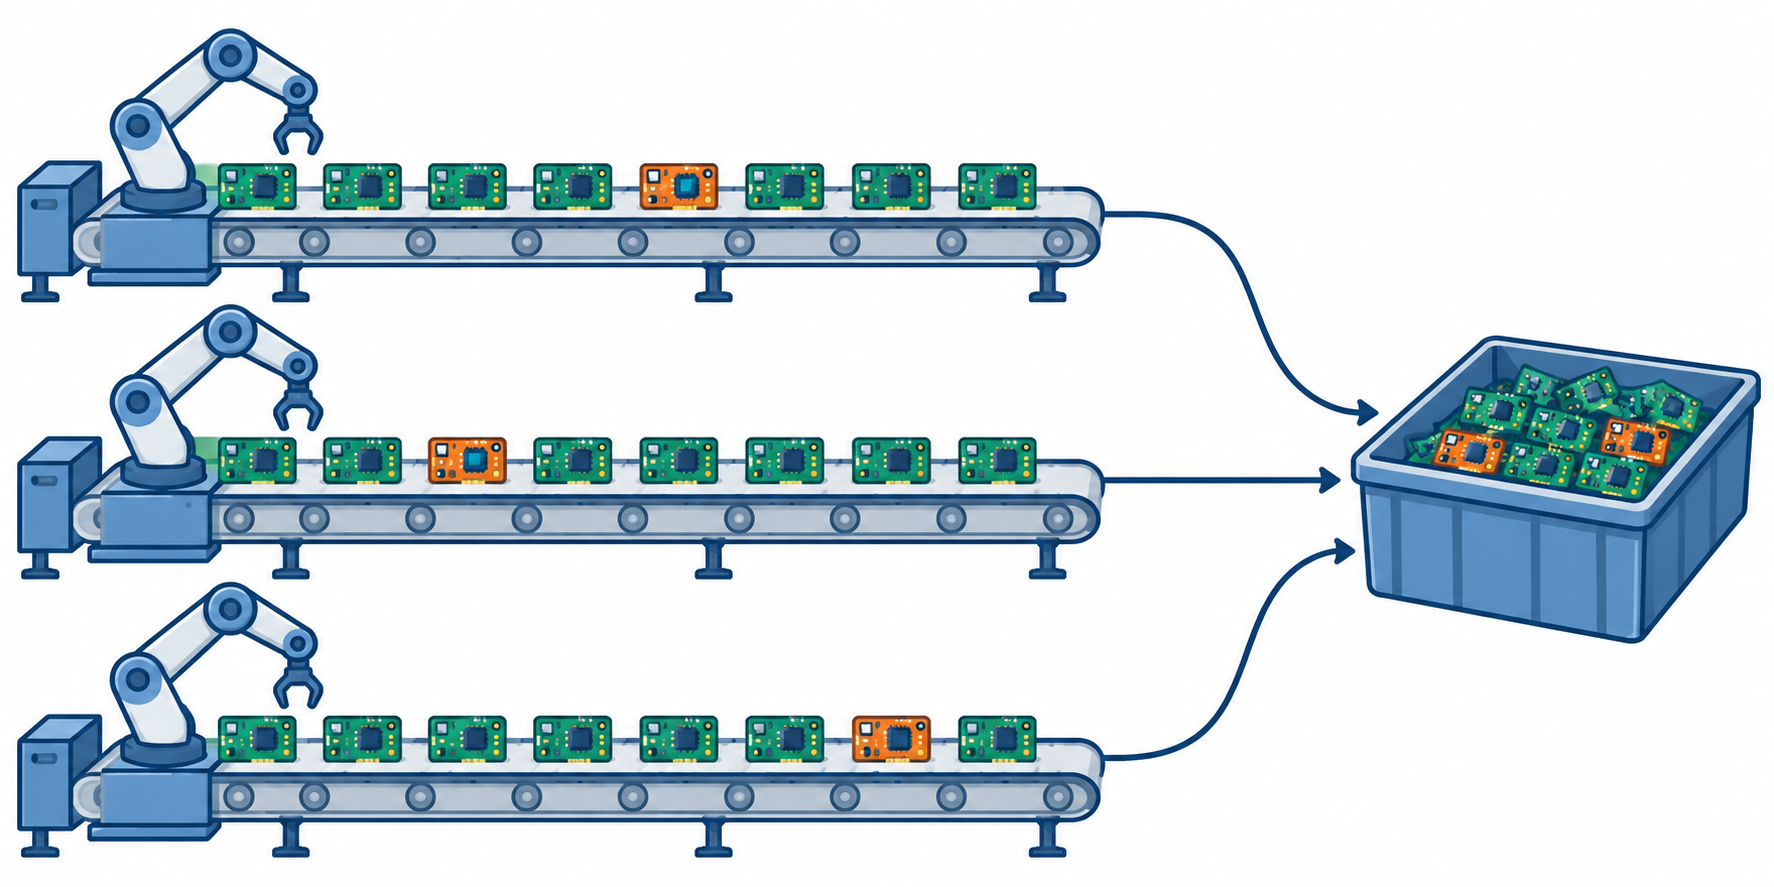
\includegraphics[width=0.42\linewidth,height=3.2cm,keepaspectratio]{images/phan3_cau5_daychuyen.png}
\end{center}

\item Một đội kiểm tra an toàn thực phẩm của Sở Y tế xét nghiệm chất cấm trong các mẫu thực phẩm tại chợ đầu mối. Thực tế có $10\%$ số mẫu thực phẩm vi phạm dư lượng chất cấm. Bộ kit thử nhanh có độ chính xác $95\%$ đối với mẫu vi phạm (dương tính thật) và có tỉ lệ báo sai $5\%$ đối với mẫu an toàn (dương tính giả). Lấy ngẫu nhiên một mẫu thực phẩm để xét nghiệm. Nếu bộ kit thử báo mẫu này vi phạm (dương tính), tính xác suất để mẫu thực phẩm đó thực sự chứa chất cấm vượt mức cho phép (làm tròn kết quả đến chữ số thập phân thứ nhất dưới dạng $\%$, ví dụ điền $67{,}9$).
\begin{center}
    
\includegraphics[width=0.42\linewidth,height=3.2cm,keepaspectratio]{images/phan3_cau6_kitthucpham.png}
\end{center}

\end{enumerate}

\newpage
% ==========================================
% BẢNG ĐÁP ÁN TỔNG HỢP
% ==========================================
\section*{BẢNG ĐÁP ÁN TỔNG HỢP}

\subsection*{1. PHẦN I}
\begin{center}
\begin{tabular}{|c|c||c|c||c|c||c|c|}
\hline
\textbf{Câu} & \textbf{Đáp án} & \textbf{Câu} & \textbf{Đáp án} & \textbf{Câu} & \textbf{Đáp án} & \textbf{Câu} & \textbf{Đáp án} \\ \hline
1 & A & 4 & A & 7 & A & 10 & A \\ \hline
2 & B & 5 & B & 8 & A & 11 & B \\ \hline
3 & A & 6 & A & 9 & A & 12 & A \\ \hline
\end{tabular}
\end{center}

\subsection*{2. PHẦN II}
\begin{center}
\begin{tabular}{|c|c|c|c|c|}
\hline
\textbf{Câu} & \textbf{Ý a)} & \textbf{Ý b)} & \textbf{Ý c)} & \textbf{Ý d)} \\ \hline
\textbf{1} & Đúng & Đúng & Đúng & Sai \\ \hline
\textbf{2} & Đúng & Sai & Đúng & Đúng \\ \hline
\textbf{3} & Đúng & Đúng & Đúng & Đúng \\ \hline
\textbf{4} & Đúng & Đúng & Đúng & Đúng \\ \hline
\end{tabular}
\end{center}

\subsection*{3. PHẦN III}
\begin{center}
\begin{tabular}{|c|c||c|c||c|c|}
\hline
\textbf{Câu} & \textbf{Kết quả điền} & \textbf{Câu} & \textbf{Kết quả điền} & \textbf{Câu} & \textbf{Kết quả điền} \\ \hline
\textbf{1} & 4 & \textbf{3} & 3,21 & \textbf{5} & 0,29 \\ \hline
\textbf{2} & 58 & \textbf{4} & 30 & \textbf{6} & 67,9 \\ \hline
\end{tabular}
\end{center}

\newpage
% ==========================================
% LỜI GIẢI CHI TIẾT
% ==========================================
\section*{HƯỚNG DẪN GIẢI CHI TIẾT}

\subsection*{PHẦN I}
\begin{enumerate}[label=\textbf{Câu \arabic*:}, leftmargin=*]
\item \textbf{Đáp án A.} Tập xác định: $D = \mathbb{R} \setminus \{1\}$. Ta có phân tích:
$y = \dfrac{x^2 - (m+2)x + 2m}{x - 1} = x - (m + 1) + \dfrac{m - 1}{x - 1}$.\\
Đạo hàm: $y' = 1 - \dfrac{m - 1}{(x - 1)^2} = \dfrac{(x - 1)^2 - (m - 1)}{(x - 1)^2}$.\\
Đồ thị $(C_m)$ có hai điểm cực trị khi và chỉ khi $y' = 0$ có hai nghiệm phân biệt khác $1 \iff m - 1 > 0 \iff m > 1$.\\
Khi đó, hoành độ hai điểm cực trị $x_1, x_2$ là hai nghiệm phân biệt của phương trình:
$(x - 1)^2 - (m - 1) = 0 \iff x^2 - 2x + 2 - m = 0$.\\
Theo định lý Vi-ét: $\left\{\begin{aligned} x_1 + x_2 &= 2 \\ x_1 x_2 &= 2 - m \end{aligned}\right.$\\
Đường thẳng đi qua hai điểm cực trị $A, B$ có phương trình:
$y = \dfrac{[x^2 - (m+2)x + 2m]'}{(x - 1)'} = 2x - m - 2$.\\
Tọa độ hai điểm cực trị là $A(x_1; 2x_1 - m - 2)$ và $B(x_2; 2x_2 - m - 2)$.\\
Tam giác $OAB$ vuông tại gốc tọa độ $O$ khi và chỉ khi $\overrightarrow{OA} \cdot \overrightarrow{OB} = 0$:\\
$\iff x_1 x_2 + y_1 y_2 = 0 \iff x_1 x_2 + [2x_1 - (m + 2)][2x_2 - (m + 2)] = 0$\\
$\iff x_1 x_2 + 4x_1 x_2 - 2(m + 2)(x_1 + x_2) + (m + 2)^2 = 0$\\
$\iff 5x_1 x_2 - 2(m + 2)(x_1 + x_2) + (m + 2)^2 = 0$\\
$\iff 5(2 - m) - 4(m + 2) + (m + 2)^2 = 0 \iff 10 - 5m - 4m - 8 + m^2 + 4m + 4 = 0$\\
$\iff m^2 - 5m + 6 = 0 \iff \left[\begin{aligned} m &= 2 \\ m &= 3 \end{aligned}\right.$\\
So sánh với điều kiện $m > 1$, cả hai giá trị $m = 2$ và $m = 3$ đều thỏa mãn. Do đó tập hợp $S = \{2; 3\}$.\\
Tổng các phần tử của tập hợp $S$ là $2 + 3 = 5$.

\item \textbf{Đáp án B.} Điều kiện để $\log_3(x^2 + 2x + m)$ xác định với mọi $x \in \mathbb{R}$ là:
$x^2 + 2x + m > 0, \, \forall x \in \mathbb{R} \iff \Delta' = 1 - m < 0 \iff m > 1$.\\
Bất phương trình trở thành:
$\log_3[3(x^2 + 1)] \ge \log_3(x^2 + 2x + m) \iff 3x^2 + 3 \ge x^2 + 2x + m \iff 2x^2 - 2x + 3 \ge m, \, \forall x \in \mathbb{R}$.\\
Xét tam thức $g(x) = 2x^2 - 2x + 3$. Ta có $\min_{\mathbb{R}} g(x) = g\left(\dfrac{1}{2}\right) = \dfrac{5}{2}$.\\
Bất phương trình nghiệm đúng với mọi $x \in \mathbb{R}$ khi và chỉ khi $m \le \min_{\mathbb{R}} g(x) = \dfrac{5}{2}$.\\
Kết hợp điều kiện xác định: $1 < m \le \dfrac{5}{2} = 2{,}5$.\\
Vì $m \in \mathbb{Z}$ và $m \in [-20; 20]$ nên chỉ có duy nhất giá trị $m = 2$. Vậy có đúng $1$ giá trị nguyên.

\item \textbf{Đáp án A.} Nhận xét: $[x f(x)]' = f(x) + x f'(x) = (x + 1)e^x$.\\
Lấy nguyên hàm hai vế:
$x f(x) = \int (x + 1)e^x dx = x e^x + C$.\\
Thay $x = 1$ vào: $1 \cdot f(1) = 1 \cdot e^1 + C \implies e = e + C \implies C = 0$.\\
Suy ra $x f(x) = x e^x \implies f(x) = e^x$ với mọi $x \in [0; 1]$.\\
Khi đó $f(x)$ liên tục và dương trên $[0; 1]$, thỏa mãn $f(1) = e$.\\
Tích phân cần tính: $I = \int_0^1 f(x) dx = \int_0^1 e^x dx = \left[ e^x \right]_0^1 = e - 1$.

\item \textbf{Đáp án A.} Mặt cầu $(S)$ có phương trình $(x - 1)^2 + (y + 2)^2 + (z - 3)^2 = 9 \implies$ tâm $I(1; -2; 3)$ và bán kính $R = 3$.\\
Gọi $K$ là điểm thỏa mãn $\overrightarrow{KA} + 2\overrightarrow{KB} = \vec{0} \implies K = \dfrac{A + 2B}{3} = \left(\dfrac{5}{3}; -\dfrac{2}{3}; \dfrac{5}{3}\right)$.\\
Biến đổi biểu thức $P$:
$P = (\overrightarrow{MK} + \overrightarrow{KA})^2 + 2(\overrightarrow{MK} + \overrightarrow{KB})^2 = 3MK^2 + KA^2 + 2KB^2 + 2\overrightarrow{MK} \cdot (\overrightarrow{KA} + 2\overrightarrow{KB}) = 3MK^2 + KA^2 + 2KB^2$.\\
Vì $KA^2 + 2KB^2$ là hằng số nên $P$ đạt GTNN khi và chỉ khi $MK$ ngắn nhất.\\
Ta có $\overrightarrow{IK} = \left(\dfrac{2}{3}; \dfrac{4}{3}; -\dfrac{4}{3}\right) \implies IK = \sqrt{\left(\dfrac{2}{3}\right)^2 + \left(\dfrac{4}{3}\right)^2 + \left(-\dfrac{4}{3}\right)^2} = 2 < R = 3$.\\
Do đó điểm $K$ nằm phía trong mặt cầu $(S)$. Khi đó điểm $M \in (S)$ gần $K$ nhất chính là giao điểm của tia $IK$ với mặt cầu $(S)$:\\
$M = I + \dfrac{R}{IK} \overrightarrow{IK} = (1; -2; 3) + \dfrac{3}{2}\left(\dfrac{2}{3}; \dfrac{4}{3}; -\dfrac{4}{3}\right) = (2; 0; 1)$.\\
Vậy $a = 2, b = 0, c = 1 \implies T = a + b + c = 2 + 0 + 1 = 3$.

\item \textbf{Đáp án B.} Ta có $u_2 \cdot u_4 = u_3^2 = 16 \implies u_3 = 4$ (vì các số hạng đều dương).\\
Theo tính chất cấp số nhân: $u_1 = \dfrac{u_3}{q^2} = \dfrac{4}{q^2}$ và $u_5 = u_3 q^2 = 4q^2$.\\
Biểu thức $P = 16u_1 + u_5 = 16 \cdot \dfrac{4}{q^2} + 4q^2 = \dfrac{64}{q^2} + 4q^2$.\\
Áp dụng bất đẳng thức Cauchy cho hai số dương $\dfrac{64}{q^2}$ và $4q^2$:\\
$P = \dfrac{64}{q^2} + 4q^2 \ge 2\sqrt{\dfrac{64}{q^2} \cdot 4q^2} = 2\sqrt{256} = 32$.\\
Đẳng thức xảy ra khi và chỉ khi $\dfrac{64}{q^2} = 4q^2 \iff q^4 = 16 \iff q = 2$ (do $q > 0$).\\
Vậy $P$ đạt giá trị nhỏ nhất khi công bội $q = 2$.

\item \textbf{Đáp án A.} Cỡ mẫu $n = 100$.\\
Tứ phân vị thứ nhất $Q_1$: do $\dfrac{n}{4} = 25$ và tần số tích lũy của nhóm $[10; 15)$ là $12 < 25$, nhóm $[15; 20)$ là $40 \ge 25$, nên nhóm chứa $Q_1$ là $[15; 20)$.\\
$Q_1 = 15 + \dfrac{25 - 12}{28} \times (20 - 15) = 15 + \dfrac{65}{28} \approx 17{,}3214\text{ phút}$.\\
Tứ phân vị thứ ba $Q_3$: do $\dfrac{3n}{4} = 75$ và tần số tích lũy của nhóm $[20; 25)$ là $12 + 28 + 35 = 75 \ge 75$, nên nhóm chứa $Q_3$ là $[20; 25)$.\\
$Q_3 = 20 + \dfrac{75 - 40}{35} \times (25 - 20) = 20 + \dfrac{35}{35} \times 5 = 25\text{ phút}$.\\
Khoảng tứ phân vị: $\Delta_Q = Q_3 - Q_1 = 25 - 17{,}3214 = 7{,}6786 \approx 7{,}68\text{ phút}$.

\item \textbf{Đáp án A.} Gọi biến cố $A_1$: "sản phẩm lấy từ dây chuyền I là phế phẩm", $P(A_1) = 0{,}03 \implies P(\overline{A_1}) = 0{,}97$.\\
Lấy 2 sản phẩm từ dây chuyền II độc lập, mỗi sản phẩm có xác suất là phế phẩm bằng $0{,}05$, không phải phế phẩm bằng $0{,}95$.\\
Để trong 3 sản phẩm lấy ra có đúng 1 phế phẩm, ta xét hai trường hợp xung khắc:\\
- TH1: Sản phẩm từ dây chuyền I là phế phẩm, 2 sản phẩm từ dây chuyền II không hỏng:\\
$P_1 = 0{,}03 \times (0{,}95)^2 = 0{,}027075$.\\
- TH2: Sản phẩm từ dây chuyền I không hỏng, đúng 1 trong 2 sản phẩm từ dây chuyền II là phế phẩm:\\
$P_2 = 0{,}97 \times C_2^1 \times 0{,}05 \times 0{,}95 = 0{,}09215$.\\
Xác suất cần tìm: $P = P_1 + P_2 = 0{,}027075 + 0{,}09215 = 0{,}119225 \approx 0{,}1192$.

\item \textbf{Đáp án A.} Mẫu số phân tích thành $(x - 2)(x - m)$.\\
Tập xác định của tử số: $x^2 - 4 \ge 0 \iff x \in (-\infty; -2] \cup [2; +\infty)$.\\
Khi $x \to \pm\infty$, ta có $\lim_{x \to \pm\infty} y = 0$ nên đồ thị hàm số luôn có duy nhất $1$ đường tiệm cận ngang $y = 0$.\\
Để đồ thị có đúng $3$ đường tiệm cận thì đồ thị phải có đúng $2$ đường tiệm cận đứng phân biệt.\\
- Tại $x = 2$: Ta có $\lim_{x \to 2^+} y = \lim_{x \to 2^+} \dfrac{\sqrt{x+2}}{\sqrt{x-2}(x-m)} = \infty$ với mọi $m \neq 2$. (Nếu $m = 2$ thì mẫu chỉ có 1 nghiệm $x = 2$, đồ thị chỉ có 1 TCĐ $x = 2 \implies$ tổng có 2 tiệm cận, loại $m = 2$).\\
- Đường thẳng $x = m$ là tiệm cận đứng thứ hai phân biệt khi và chỉ khi $m \neq 2$ và $x = m$ thuộc tập xác định của hàm số (tức $m \le -2$ hoặc $m > 2$).\\
Do $m \in [-10; 10], m \in \mathbb{Z}$:\\
+ $m \le -2 \implies m \in \{-10, -9, \dots, -2\}$: có 9 giá trị.\\
+ $m > 2 \implies m \in \{3, 4, \dots, 10\}$: có 8 giá trị.\\
Tổng số giá trị nguyên của $m$ là $9 + 8 = 17$ giá trị.

\item \textbf{Đáp án A.} Thể tích khối tròn xoay tạo thành khi quay $(H)$ quanh trục $Ox$ là:
$V = \pi \int_0^1 y^2 dx = \pi \int_0^1 x^2 \ln(x + 1) dx$.\\
Đặt $\left\{\begin{aligned} u &= \ln(x + 1) \\ dv &= x^2 dx \end{aligned}\right. \implies \left\{\begin{aligned} du &= \dfrac{1}{x + 1} dx \\ v &= \dfrac{x^3}{3} \end{aligned}\right.$\\
Áp dụng công thức tích phân từng phần:
\begin{align*}
V &= \pi \left( \left[ \dfrac{x^3}{3} \ln(x + 1) \right]_0^1 - \dfrac{1}{3} \int_0^1 \dfrac{x^3}{x + 1} dx \right) \\
&= \pi \left( \dfrac{1}{3} \ln 2 - \dfrac{1}{3} \int_0^1 \left( x^2 - x + 1 - \dfrac{1}{x + 1} \right) dx \right) \\
&= \pi \left( \dfrac{1}{3} \ln 2 - \dfrac{1}{3} \left[ \dfrac{x^3}{3} - \dfrac{x^2}{2} + x - \ln(x + 1) \right]_0^1 \right) \\
&= \pi \left( \dfrac{1}{3} \ln 2 - \dfrac{1}{3} \left( \dfrac{5}{6} - \ln 2 \right) \right) = \pi \left( \dfrac{2}{3} \ln 2 - \dfrac{5}{18} \right).
\end{align*}

\item \textbf{Đáp án A.} Đường thẳng $d_1$ đi qua $M_1(1; -1; 0)$ có VTCP $\vec{u}_1 = (2; 1; -1)$.\\
Đường thẳng $d_2$ đi qua $M_2(2; 3; -1)$ có VTCP $\vec{u}_2 = (1; -2; 2)$.\\
Tích có hướng $[\vec{u}_1, \vec{u}_2] = (1 \cdot 2 - (-1)(-2); \, (-1) \cdot 1 - 2 \cdot 2; \, 2(-2) - 1 \cdot 1) = (0; -5; -5)$.\\
Độ dài $|[\vec{u}_1, \vec{u}_2]| = \sqrt{0^2 + (-5)^2 + (-5)^2} = 5\sqrt{2}$.\\
Vectơ $\overrightarrow{M_1 M_2} = (2 - 1; 3 - (-1); -1 - 0) = (1; 4; -1)$.\\
Khoảng cách giữa hai đường thẳng chéo nhau $d_1$ và $d_2$ là:\\
$d(d_1, d_2) = \dfrac{|[\vec{u}_1, \vec{u}_2] \cdot \overrightarrow{M_1 M_2}|}{|[\vec{u}_1, \vec{u}_2]|} = \dfrac{|0(1) - 5(4) - 5(-1)|}{5\sqrt{2}} = \dfrac{|-15|}{5\sqrt{2}} = \dfrac{3}{\sqrt{2}} = \dfrac{3\sqrt{2}}{2}$.

\item \textbf{Đáp án B.} Đặt $t = 3^x$. Vì $x \in [0; 1]$ nên $t \in [1; 3]$.\\
Bất phương trình trở thành: $t^2 - 3mt + 2m + 1 \le 0 \iff m(3t - 2) \ge t^2 + 1$.\\
Vì $t \in [1; 3]$ nên $3t - 2 \ge 3(1) - 2 = 1 > 0$, do đó $m \ge \dfrac{t^2 + 1}{3t - 2} = g(t)$.\\
Bất phương trình có nghiệm thuộc $[0; 1]$ khi và chỉ khi $m \ge \min_{t \in [1; 3]} g(t)$.\\
Đạo hàm $g'(t) = \dfrac{2t(3t - 2) - 3(t^2 + 1)}{(3t - 2)^2} = \dfrac{3t^2 - 4t - 3}{(3t - 2)^2}$.\\
Trên đoạn $[1; 3]$, $g'(t) = 0 \iff t = \dfrac{2 + \sqrt{13}}{3} \approx 1{,}87$.\\
Ta có $g(1) = 2$, $g(3) = \dfrac{10}{7} \approx 1{,}43$, và $g\left(\dfrac{2 + \sqrt{13}}{3}\right) = \dfrac{4 + 2\sqrt{13}}{9} \approx 1{,}25$.\\
Do đó $\min_{t \in [1; 3]} g(t) \approx 1{,}25 \implies m \ge 1{,}25$.\\
Vì $m \in \mathbb{Z}$ và $m \in [-10; 10]$ nên $m \in \{2, 3, 4, 5, 6, 7, 8, 9, 10\}$.\\
Số giá trị nguyên thỏa mãn là $10 - 2 + 1 = 9$ giá trị.

\item \textbf{Đáp án A.} Gọi $I$ là trung điểm của đoạn thẳng $AB \implies I(2; 1; 0)$.\\
Áp dụng công thức độ dài đường trung tuyến:\\
$P = MA^2 + MB^2 = (\overrightarrow{MI} + \overrightarrow{IA})^2 + (\overrightarrow{MI} + \overrightarrow{IB})^2 = 2MI^2 + IA^2 + IB^2 + 2\overrightarrow{MI} \cdot (\overrightarrow{IA} + \overrightarrow{IB}) = 2MI^2 + \dfrac{AB^2}{2}$.\\
Vì hai điểm $A, B$ cố định nên $P$ đạt giá trị nhỏ nhất khi và chỉ khi khoảng cách $MI$ ngắn nhất, tức $M$ là hình chiếu vuông góc của trung điểm $I$ lên đường thẳng $d$.\\
Điểm $M \in d \implies M(1 + t; 2t; -1 - 2t) \implies \overrightarrow{IM} = (t - 1; 2t - 1; -2t - 1)$.\\
Đường thẳng $d$ có VTCP $\vec{u}_d = (1; 2; -2)$.\\
Điều kiện vuông góc: $\overrightarrow{IM} \cdot \vec{u}_d = 0 \iff 1(t - 1) + 2(2t - 1) - 2(-2t - 1) = 0$\\
$\iff t - 1 + 4t - 2 + 4t + 2 = 0 \iff 9t - 1 = 0 \iff t = \dfrac{1}{9}$.\\
Thay $t = \dfrac{1}{9}$ vào tọa độ điểm $M$ ta được: $M\left(\dfrac{10}{9}; \dfrac{2}{9}; -\dfrac{11}{9}\right)$.
\end{enumerate}

\subsection*{PHẦN II}
\begin{enumerate}[label=\textbf{Câu \arabic*:}, leftmargin=*]
\item \textbf{Câu 1 (Tối ưu Kinh tế):}
\begin{itemize}
    \item a) \textbf{Đúng}: Doanh thu $R(x) = x \cdot p(x) = x(100 - 2x) = 100x - 2x^2$ (triệu đồng).
    \item b) \textbf{Đúng}: Lợi nhuận $L(x) = R(x) - C(x) = (100x - 2x^2) - (0{,}1x^3 - 3x^2 + 40x + 100) = -0{,}1x^3 + x^2 + 60x - 100$.
    \item c) \textbf{Đúng}: Với $x = 10$, ta có $L(10) = -0{,}1(10^3) + 10^2 + 60(10) - 100 = -100 + 100 + 600 - 100 = 500$ triệu đồng.
    \item d) \textbf{Sai}: $L'(x) = -0{,}3x^2 + 2x + 60 = 0 \implies x = \dfrac{10 + \sqrt{1900}}{3} \approx 17{,}86\text{ tấn} \neq 18\text{ tấn}$. Mặt khác, tại $x = 18$ thì $L(18) = -0{,}1(18^3) + 18^2 + 60(18) - 100 = 720{,}8$ triệu đồng $\neq 718{,}8$ triệu đồng.
\end{itemize}

\item \textbf{Câu 2 (Thu Năng lượng Mặt trời):}
\begin{itemize}
    \item a) \textbf{Đúng}: Đạo hàm $f'(t) = -0{,}3t + 1{,}8 = 0 \iff t = 6$ (tương ứng $12$ giờ trưa). Vì $f''(t) = -0{,}3 < 0$ nên tốc độ thu năng lượng đạt cực đại tại $t = 6$.
    \item b) \textbf{Sai}: $F(6) = \int_0^6 (-0{,}15t^2 + 1{,}8t) dt = \left[-0{,}05t^3 + 0{,}9t^2\right]_0^6 = -10{,}8 + 32{,}4 = 21{,}6\text{ kWh} \neq 16{,}2\text{ kWh}$.
    \item c) \textbf{Đúng}: $F(12) = \int_0^{12} (-0{,}15t^2 + 1{,}8t) dt = \left[-0{,}05t^3 + 0{,}9t^2\right]_0^{12} = -86{,}4 + 129{,}6 = 43{,}2\text{ kWh}$.
    \item d) \textbf{Đúng}: Lượng năng lượng $80\%$ của cả ngày là $0{,}8 \times 43{,}2 = 34{,}56\text{ kWh}$. Giải phương trình $-0{,}05t^3 + 0{,}9t^2 = 34{,}56$ trên $[0; 12]$ ta được nghiệm $t \approx 8{,}55\text{ giờ}$ (khoảng 8 giờ 33 phút). Thời điểm tương ứng là $6\text{h} + 8\text{h}33\text{p} = 14\text{h}33\text{p}$, tức khoảng 14 giờ 30 phút.
\end{itemize}

\item \textbf{Câu 3 (Chẩn đoán AI \& Bayes):}
\begin{itemize}
    \item a) \textbf{Đúng}: Xác suất không mắc bệnh là $P(\overline{A}) = 1 - P(A) = 1 - 0{,}005 = 0{,}995$ ($99{,}5\%$).
    \item b) \textbf{Đúng}: Theo công thức xác suất toàn phần: $P(B) = P(A)P(B|A) + P(\overline{A})P(B|\overline{A}) = 0{,}005 \times 0{,}96 + 0{,}995 \times 0{,}02 = 0{,}0048 + 0{,}0199 = 0{,}0247$ ($2{,}47\%$).
    \item c) \textbf{Đúng}: Theo công thức Bayes: $P(A|B) = \dfrac{P(A \cap B)}{P(B)} = \dfrac{0{,}0048}{0{,}0247} \approx 19{,}43\% \approx 19{,}4\%$.
    \item d) \textbf{Đúng}: Xác suất có bệnh sau vòng 1 là $p_1 \approx 0{,}1943$. Với xét nghiệm chuyên sâu có độ nhạy $98\%$ và tỉ lệ âm tính giả $2\%$ (dương tính giả $2\%$):
    \begin{align*}
    P(\text{mắc bệnh} \mid +_2) &= \dfrac{0{,}1943 \times 0{,}98}{0{,}1943 \times 0{,}98 + (1 - 0{,}1943) \times 0{,}02} \\
    &\approx \dfrac{0{,}1904}{0{,}1904 + 0{,}0161} \approx 92{,}2\% > 90\%.
    \end{align*}
\end{itemize}

\item \textbf{Câu 4 (Treo Tấm Sàn Bê Tông):}
\begin{itemize}
    \item a) \textbf{Đúng}: Tọa độ $S(0; 0; 6), A(-2; -3; 0) \implies \overrightarrow{SA} = (-2; -3; -6)$.\\
    Độ dài $|\overrightarrow{SA}| = \sqrt{(-2)^2 + (-3)^2 + (-6)^2} = 7\text{ m}$.
    \item b) \textbf{Đúng}: Tương tự, $|\overrightarrow{SB}| = |\overrightarrow{SC}| = |\overrightarrow{SD}| = \sqrt{2^2 + 3^2 + 6^2} = 7\text{ m}$.
    \item c) \textbf{Đúng}: Các sợi dây tác dụng lực kéo lên sàn hướng về phía điểm treo $S$. Vectơ đơn vị hướng dọc theo dây $SA$ từ $A$ lên $S$ là $\vec{u} = \left(\dfrac{2}{7}; \dfrac{3}{7}; \dfrac{6}{7}\right)$. Hình chiếu thẳng đứng của lực căng mỗi dây là $F_z = F \cdot \dfrac{6}{7}$. Do 4 dây chịu lực đối xứng, cân bằng với trọng lực $\vec{P} = (0; 0; -3000)\text{ N}$:\\
    $4 \cdot F \cdot \dfrac{6}{7} = 3000 \implies F = \dfrac{3000 \times 7}{24} = 875\text{ N}$.
    \item d) \textbf{Đúng}: Mặt phẳng sàn $(ABCD)$ là mặt phẳng $Oxy$. Sin của góc $\alpha$ giữa đường thẳng $SA$ và mặt phẳng sàn bằng $|\cos(\overrightarrow{SA}, \vec{k})| = \dfrac{6}{7} \implies \alpha = \arcsin\left(\dfrac{6}{7}\right) \approx 59^\circ$.
\end{itemize}
\end{enumerate}

\subsection*{PHẦN III}
\begin{enumerate}[label=\textbf{Câu \arabic*:}, leftmargin=*]
\item \textbf{Đáp số: 4.} Gọi chiều rộng đáy bể là $w$ (m, $w > 0$), khi đó chiều dài đáy là $2w$ (m).\\
Gọi chiều cao của bể là $h$ (m, $h > 0$).\\
Thể tích bể: $V = 2w \cdot w \cdot h = 2w^2 h = 72 \implies h = \dfrac{36}{w^2}$.\\
Diện tích đáy: $S_{\text{đáy}} = 2w^2$; diện tích nắp: $S_{\text{nắp}} = 2w^2$; diện tích bốn mặt xung quanh: $S_{xq} = 2(2wh) + 2(wh) = 6wh$.\\
Tổng chi phí làm bể (triệu đồng):\\
$C(w) = 1 \cdot S_{\text{đáy}} + 1 \cdot S_{\text{nắp}} + 1 \cdot S_{xq} = 4w^2 + 6wh = 4w^2 + 6w \cdot \dfrac{36}{w^2} = 4w^2 + \dfrac{216}{w}$.\\
Xét hàm số $C(w)$ trên khoảng $(0; +\infty)$:\\
$C'(w) = 8w - \dfrac{216}{w^2} = 0 \iff 8w^3 = 216 \iff w^3 = 27 \iff w = 3\text{ m}$.\\
Bảng biến thiên cho thấy $C(w)$ đạt giá trị nhỏ nhất tại $w = 3\text{ m}$.\\
Khi đó chiều cao tương ứng của bể là $h = \dfrac{36}{3^2} = \dfrac{36}{9} = 4\text{ m}$.

\item \textbf{Đáp số: 58.} Gọi $A = 15$ triệu đồng là số tiền gửi đều đặn đầu mỗi tháng, lãi suất $r = 0{,}5\% = 0{,}005$/tháng.\\
Sau $n$ tháng, tổng số tiền cả gốc lẫn lãi tích lũy được ngay sau khi tính lãi tháng thứ $n$ là:\\
$S_n = A(1 + r) + A(1 + r)^2 + \dots + A(1 + r)^n = A(1 + r) \dfrac{(1 + r)^n - 1}{r}$.\\
Để số tiền vượt quá $1$ tỷ đồng ($1000$ triệu đồng):\\
$15(1{,}005) \dfrac{(1{,}005)^n - 1}{0{,}005} > 1000 \iff (1{,}005)^n - 1 > \dfrac{1000 \times 0{,}005}{15 \times 1{,}005} \approx 0{,}331675$\\
$\iff (1{,}005)^n > 1{,}331675 \iff n > \dfrac{\ln(1{,}331675)}{\ln(1{,}005)} \approx 57{,}43$.\\
Vì số tháng gửi là số nguyên nên sau ít nhất $n = 58$ tháng (tức $4$ năm $10$ tháng) thì số tiền tích lũy vượt quá $1$ tỷ đồng.

\item \textbf{Đáp số: 3,21.} Tọa độ vị trí của hai drone tại thời điểm $t$ là $A(1 + 2t; 2 + t; 3 + t)$ và $B(5 + t; 1 + 3t; 1 + 2t)$.\\
Vectơ $\overrightarrow{AB}(t) = (4 - t; -1 + 2t; -2 + t)$.\\
Bình phương khoảng cách giữa hai drone là:\\
$d^2(t) = (4 - t)^2 + (2t - 1)^2 + (t - 2)^2 = 6t^2 - 16t + 21$.\\
Tam thức bậc hai đạt cực tiểu tại $t = \dfrac{16}{2 \times 6} = \dfrac{4}{3}\text{ phút}$.\\
Khoảng cách ngắn nhất là $d_{\min} = \sqrt{6\left(\dfrac{4}{3}\right)^2 - 16\left(\dfrac{4}{3}\right) + 21} = \sqrt{\dfrac{31}{3}} \approx 3{,}2145 \approx 3{,}21\text{ km}$.

\item \textbf{Đáp số: 30.} Tổng số hợp tác xã là $60 \implies 8 + 12 + x + y + 6 = 60 \iff x + y = 34$.\\
Do $M_e = 16{,}4 \in [16; 18)$ nên nhóm chứa trung vị là $[16; 18)$.\\
Áp dụng công thức tính trung vị cho mẫu số liệu ghép nhóm:\\
$M_e = 16 + \dfrac{30 - (8 + 12 + x)}{y} \times (18 - 16) = 16 + \dfrac{2(10 - x)}{y} = 16{,}4 \iff \dfrac{10 - x}{y} = 0{,}2 = \dfrac{1}{5} \iff y = 50 - 5x$.\\
Thay vào phương trình tổng: $x + (50 - 5x) = 34 \iff 4x = 16 \iff x = 4 \implies y = 30$.

\item \textbf{Đáp số: 0,29.} Gọi $H$ là biến cố "linh kiện rút ra bị hỏng".\\
Áp dụng công thức xác suất toàn phần, xác suất lấy trúng linh kiện hỏng là:\\
$P(H) = P(D_1)P(H|D_1) + P(D_2)P(H|D_2) + P(D_3)P(H|D_3)$\\
$= 0{,}50 \times 0{,}01 + 0{,}30 \times 0{,}02 + 0{,}20 \times 0{,}03 = 0{,}005 + 0{,}006 + 0{,}006 = 0{,}017$.\\
Theo công thức Bayes, xác suất linh kiện bị hỏng này do dây chuyền $D_1$ sản xuất là:\\
$P(D_1|H) = \dfrac{P(D_1)P(H|D_1)}{P(H)} = \dfrac{0{,}50 \times 0{,}01}{0{,}017} = \dfrac{0{,}005}{0{,}017} = \dfrac{5}{17} \approx 0{,}2941 \approx 0{,}29$.

\item \textbf{Đáp số: 67,9.} Gọi $V$ là biến cố "mẫu thực phẩm vi phạm" $\implies P(V) = 0{,}10$, $P(\overline{V}) = 0{,}90$.\\
Gọi $T$ là biến cố "bộ kit thử cho kết quả dương tính (báo vi phạm)".\\
Độ chính xác đối với mẫu vi phạm: $P(T|V) = 0{,}95$.\\
Tỉ lệ báo sai đối với mẫu an toàn: $P(T|\overline{V}) = 0{,}05$.\\
Xác suất để một mẫu bất kỳ có kết quả dương tính là:\\
$P(T) = P(V)P(T|V) + P(\overline{V})P(T|\overline{V}) = 0{,}10 \times 0{,}95 + 0{,}90 \times 0{,}05 = 0{,}095 + 0{,}045 = 0{,}140$.\\
Theo công thức Bayes, xác suất mẫu thực sự vi phạm khi đã có kết quả dương tính là:\\
$P(V|T) = \dfrac{P(V)P(T|V)}{P(T)} = \dfrac{0{,}095}{0{,}140} = \dfrac{19}{28} \approx 67{,}857\% \approx 67{,}9\%$.
\end{enumerate}

\end{document}
